\documentclass[handout]{beamer}

\usepackage{minted}
\usepackage[utf8]{inputenc}
\usepackage{graphicx}
\usepackage[T1]{fontenc}

\mode<presentation>{
  \usetheme{default}
}

\setbeamertemplate{navigation symbols}{}
\setbeamertemplate{footline}[frame number]

%% -------------------------------------------------------------------------- %%

\title{A visual DSL toolkit in Lua}
\subtitle{Past, present and future}
\author{
\includegraphics[height=.4\textheight]{logo}}
\institute{Alexander Gladysh <ag@logiceditor.com>}
\date{Lua Workshop 2013\\Toulouse}

%% -------------------------------------------------------------------------- %%

\begin{document}

\maketitle

%% -------------------------------------------------------------------------- %%

\begin{frame}{Outline}

\tableofcontents

\end{frame}

%% -------------------------------------------------------------------------- %%

\section{Introduction}

%% -------------------------------------------------------------------------- %%

\begin{frame}{Alexander Gladysh}

\begin{itemize}
\item CTO, co-founder at LogicEditor
\item In löve with Lua since 2005
\end{itemize}

\end{frame}

%% -------------------------------------------------------------------------- %%

\begin{frame}{LogicEditor}

\begin{itemize}
\item Use Lua to develop:
\begin{itemize}
  \item Visual DSL toolkit (subject of this talk)
  \item Big-data analytics
  \item Intensive-load web-services
  \item In-browser and mobile games
\end{itemize}
\item 600+ KLOC of private Lua codebase
\item Some contributions to open-source Lua projects
\end{itemize}

\end{frame}

%% -------------------------------------------------------------------------- %%

\section{The Problem}

%% -------------------------------------------------------------------------- %%

\begin{frame}{The Problem}

\begin{itemize}
\item Business-logic is highly volatile.
\item Programmers are not domain area specialists.
\item Specialist $\Leftrightarrow$ Manager $\Leftrightarrow$ Programmer
loop is slow.
\item Specialist $\Leftrightarrow$ Programmer loop is expensive.
\item Let specialists do the business-logic!
\end{itemize}

\end{frame}

%% -------------------------------------------------------------------------- %%

\begin{frame}


\includegraphics[height=.8\textheight]{omgwtf}

\end{frame}

%% -------------------------------------------------------------------------- %%

\begin{frame}{Non-programmers aren't programmers}

It is not enough to be able to compose an algorithm and even implement it
with some simple programming language.

For commercial programming you'll also need, at least:

\begin{itemize}
\item Technical background
\item Debugging skills
\item Team coding skills
\end{itemize}

\end{frame}

%% -------------------------------------------------------------------------- %%

\begin{frame}{Solution}

\begin{itemize}
\item A tool that prevents \textit{technical} mistakes
\item While limiting creativity as little as possible
\item And is within grasp of a non-programmer.
\end{itemize}

\end{frame}

%% -------------------------------------------------------------------------- %%

\begin{frame}{Ad-hoc implementations}

\begin{itemize}
\item One-shot, very limited flexibility
\item Full of crutches
\item Hard to maintain
\end{itemize}

\end{frame}

%% -------------------------------------------------------------------------- %%

\section{Classic third-party alternatives}

%% -------------------------------------------------------------------------- %%

\begin{frame}

\Huge{Classic third-party alternatives}

\end{frame}

%% -------------------------------------------------------------------------- %%

\begin{frame}{MIT Scratch}

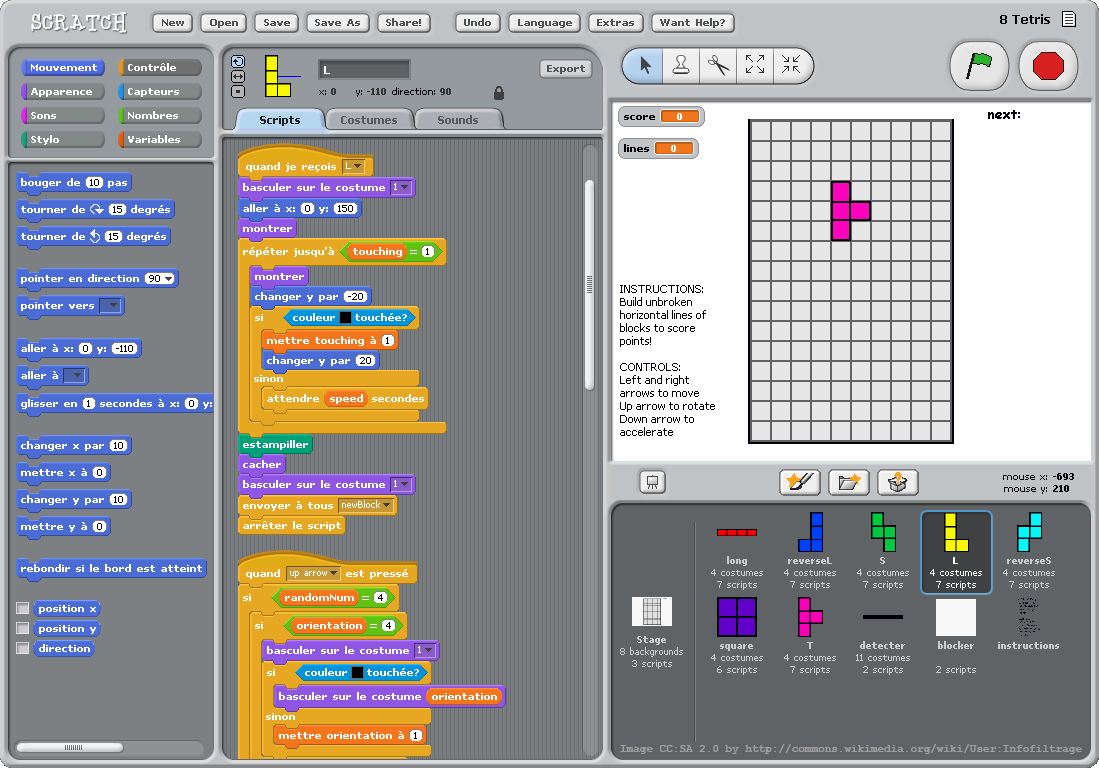
\includegraphics[height=.8\textheight]{scratch}

\end{frame}

%% -------------------------------------------------------------------------- %%

\begin{frame}{Descent Freespace Editor Events}

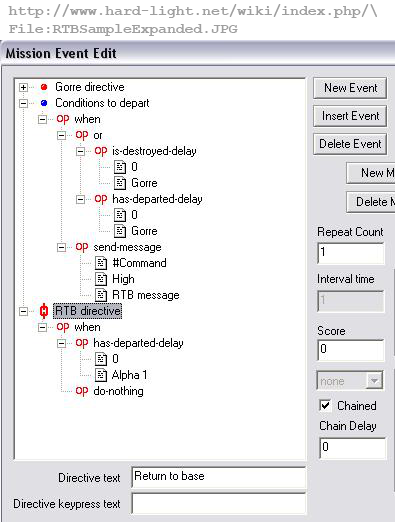
\includegraphics[height=.8\textheight]{freespace}

\end{frame}

%% -------------------------------------------------------------------------- %%

\begin{frame}{Lego NXT-G}

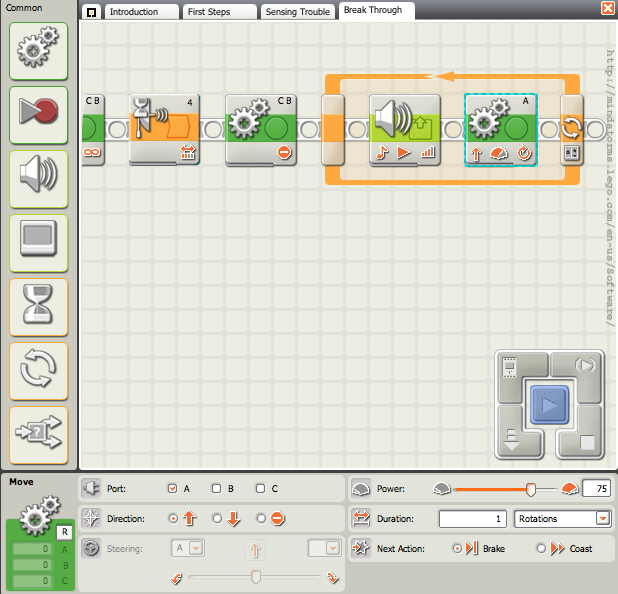
\includegraphics[height=.8\textheight]{lego}

\end{frame}

%% -------------------------------------------------------------------------- %%

\begin{frame}{Apple Automator}

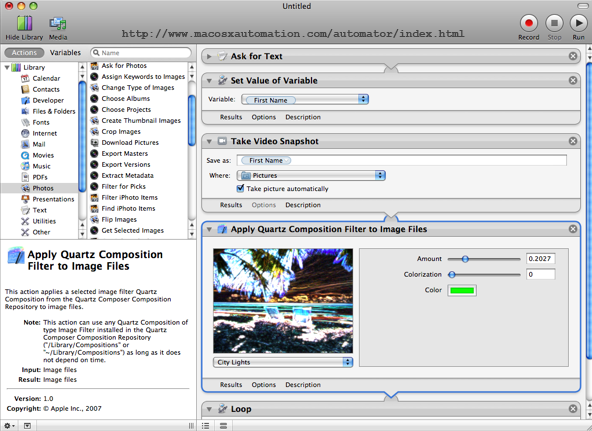
\includegraphics[height=.8\textheight]{automator}

\end{frame}

%% -------------------------------------------------------------------------- %%

\begin{frame}{What is in common?}

\begin{itemize}
\item \textbf{A visual domain-specific language},
\item that allows user to describe
\item \textbf{the control-flow}.
\end{itemize}

\end{frame}

%% -------------------------------------------------------------------------- %%

\section{Past generations}

%% -------------------------------------------------------------------------- %%

\begin{frame}{A retrospective of ideas}

Screenshots shown here are from editors done by
me and/or my colleagues for different companies
we worked for, over time.

Only an idea was re-used and improved between generations.

\end{frame}

%% -------------------------------------------------------------------------- %%

\begin{frame}{Video-adventure game editor}

(No screenshots available)

\begin{itemize}
\item Legacy, circa 2002—2004
\item Graph of in-game dialog remarks and answer choices
\item Allowing to tie-in video-loop to remark
\item No Lua.
\end{itemize}

\end{frame}

%% -------------------------------------------------------------------------- %%

\begin{frame}{Adventure game dialog editor, I, II}

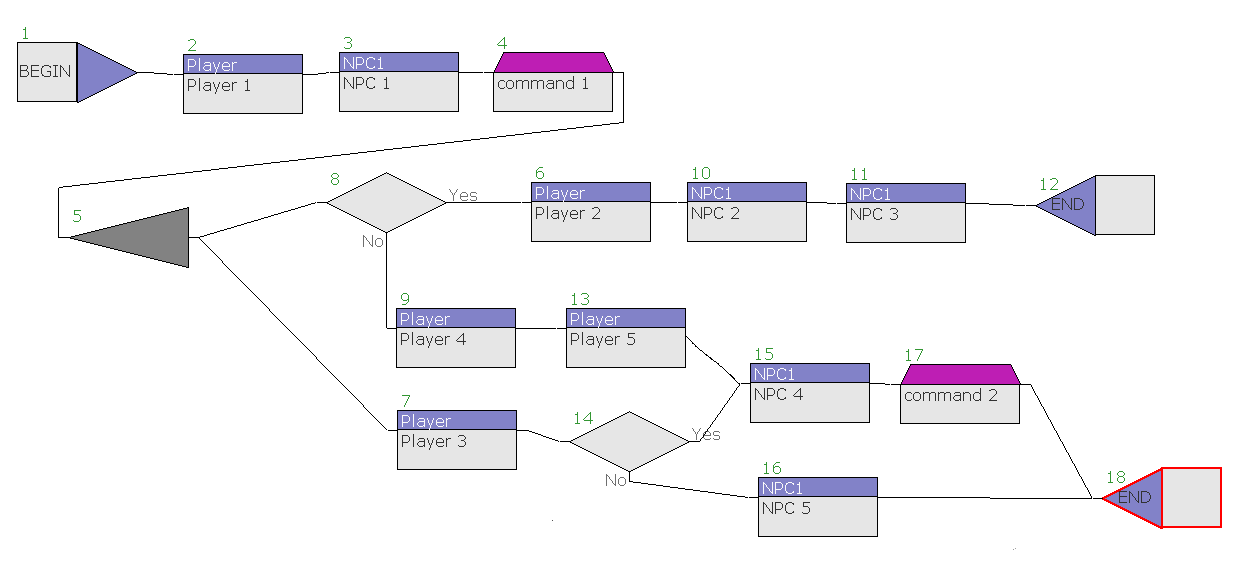
\includegraphics[height=.4\textheight]{adventure}

\begin{itemize}
\item Graph of in-game dialog remarks and answer choices
\item With ability to add custom Lua code logic (in II)
\item Generated data (in Lua) for a state machine (also in Lua)
\end{itemize}

\end{frame}

%% -------------------------------------------------------------------------- %%

\begin{frame}{Browser MMO quest editor, I, II}

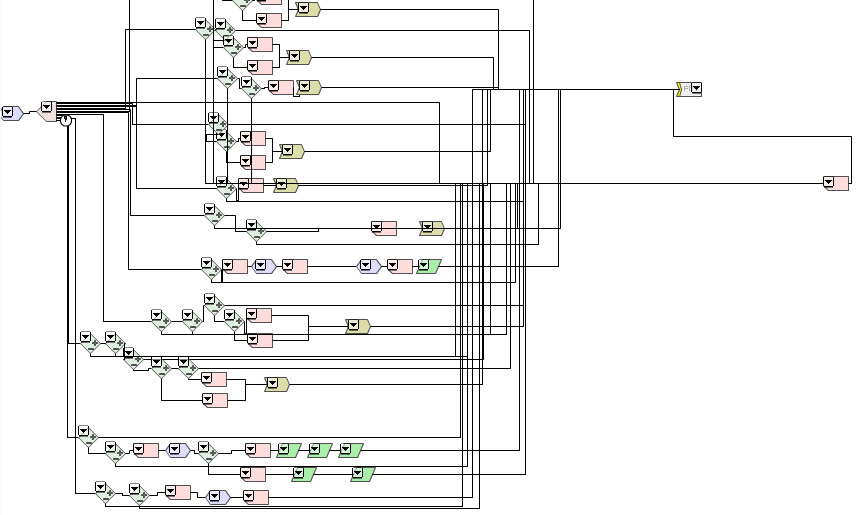
\includegraphics[height=.8\textheight]{browser}

\end{frame}

%% -------------------------------------------------------------------------- %%

\begin{frame}{Browser MMO magic system editor}

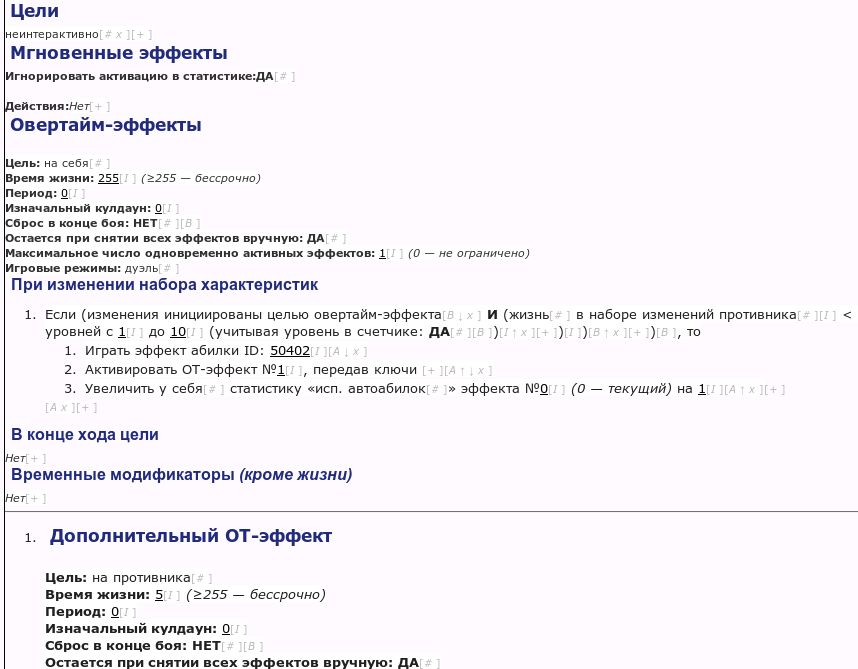
\includegraphics[height=.8\textheight]{magic}

\end{frame}

%% -------------------------------------------------------------------------- %%

\begin{frame}{Analysis}

\begin{itemize}
\item Some non-programmers prefer visual control-flow editors.
\item Some — textual representation.
\item (Programmers hate to use both kinds.)
\item All editors were very useful, some — invaluable.
\item But, in retrospective, some should have been replaced by dedicated coders.
\item None of the past-generation editors were flexible enough to be
used outside its immediate domain (but this never was an official goal
for them).
\end{itemize}

\end{frame}

%% -------------------------------------------------------------------------- %%

\section{The present generation}

%% -------------------------------------------------------------------------- %%

\begin{frame}{The Visual Business Logic Editor Toolkit}

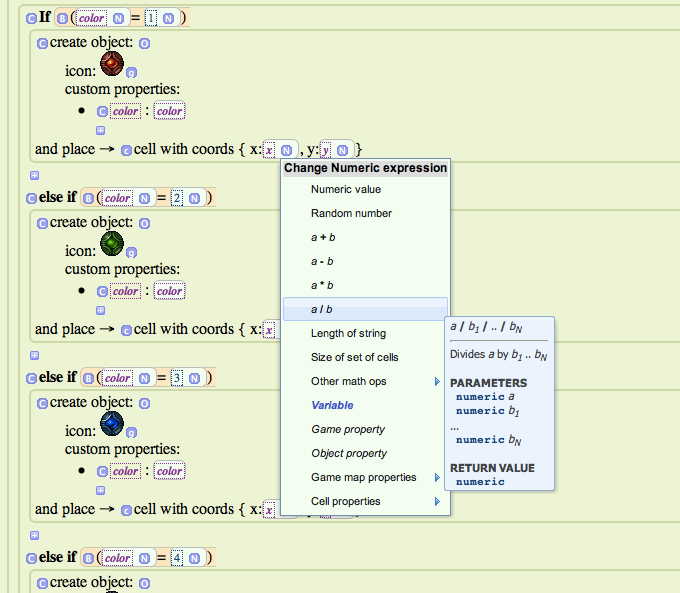
\includegraphics[height=.8\textheight]{gamector}

\end{frame}

%% -------------------------------------------------------------------------- %%

\begin{frame}{Design goals}

\begin{itemize}
\item Easy to create new editors.
\item Easy to support existing editors.
\item Easy to integrate with "any" other project on "any" technology.
\item Easy \textit{enough} to learn and use by end-users.
\end{itemize}

\end{frame}

%% -------------------------------------------------------------------------- %%

\begin{frame}{Editor use-cases}

For example:

\begin{itemize}
\item A dialog editor for a game scenario writer.
\item A magic system editor for a game-designer.
\item A mission logic editor for a game level-designer.
\item A DB query editor for a data analyst (Hadoop, anyone?).
\item An advertising campaign targeting editor for a marketer.
\item ...and so on.
\end{itemize}

\end{frame}

%% -------------------------------------------------------------------------- %%

\begin{frame}{Technology}

\begin{itemize}
\item The data is a tree corresponding to the control flow (or to
anything tree-like, actually).
\item The output is structured text (code or data).
\item Editor code, UI and backend, is generated by Lua code in the
Toolkit, from the data "schema".
\item Editor UI is in JavaScript / HTML, backend is in Lua.
\end{itemize}

\end{frame}

%% -------------------------------------------------------------------------- %%

\begin{frame}{The Data Schema}

\begin{itemize}
\item Embedded Lua DSL (see my talk on Lua WS'11).
\url{http://bit.ly/lua-dsl-talk}
\item Describes how to:
\begin{itemize}
 \item check data validity,
 \item generate default data,
 \item render data to editor UI,
 \item change data in editor UI,
 \item render the conforming data to the output code (or data).
\end{itemize}
\item Two layers: human-friendly and machine-friendly
\end{itemize}

\end{frame}

%% -------------------------------------------------------------------------- %%

\begin{frame}[fragile]{Schema Example, I}

See also: \url{http://bit.ly/le7-schema}

\begin{minted}{lua}
lang:root "lua.print-string"

lang:value "lua.string.value" {
  data_type = "string";
  default = "Hallo, world!";
  render:js [[String Value]] { [[${1}]] };
  render:lua { [[${1}]] };
}
\end{minted}

\end{frame}

%% -------------------------------------------------------------------------- %%

\begin{frame}[fragile]{Schema Example, II}

\begin{minted}{lua}
lang:func "lua.print-string" {
  "lua.string.value";
  render:js [[Print string]] {
    [[Print: ${1}]];
  };
  render:lua {
    [[print(${1})]];
  };
}

\end{minted}

\end{frame}

%% -------------------------------------------------------------------------- %%

\begin{frame}[fragile]{Default Data}

\begin{minted}{lua}
{
  id = "lua.print-string";
  {
    id = "lua.string.value";
    "Hallo, world!";
  }
}
\end{minted}

Renders to Lua as:

\begin{minted}{lua}
print("Hallo, world!")
\end{minted}

\end{frame}

%% -------------------------------------------------------------------------- %%

\begin{frame}[fragile]{UI for default data (simplified)}

\begin{minted}{lua}
<div id="lua.print-string">
  Print: <span id="lua.string.value">Hallo, world!</span>
</div>
\end{minted}

\textit{NB: That <span> turns to edit-box on click.}

\end{frame}

%% -------------------------------------------------------------------------- %%

\begin{frame}[fragile]{Extending string type}

\begin{minted}{lua}
lang:type "lua.string" {
  init = "lua.string.value";
  render:js [[String]] { menu = [[S]]; [[${1}]] };
  render:lua { [[${1}]] };
}

lang:func "lua.string.reverse" {
  type = "lua.string";
  render:js [[Reverse string]] { [[Reverse: ${1}]] };
  render:lua { [[(${1}):reverse()]] };
}
\end{minted}

\end{frame}

%% -------------------------------------------------------------------------- %%

\begin{frame}[fragile]{Print with multiple arguments}

\begin{minted}{lua}
lang:list "lua.print"
{
  "lua.string";
  render:js [[Print]] {
    empty = [[Print newline]];
    before = [[Print values: <ul><li>]];
    glue = [[</li><li>]];
    after = [[</li></ul>]];
  };
  render:lua {
    before = [[print(]];
    glue = [[,]];
    after = [[)]];
  };
}
\end{minted}

\end{frame}

%% -------------------------------------------------------------------------- %%

\begin{frame}{Main primitives}

\begin{itemize}
\item lang:const
\item lang:value
\item lang:enum
\item lang:func
\item lang:list
\item lang:type
\end{itemize}

\end{frame}

%% -------------------------------------------------------------------------- %%

\begin{frame}{Machine-friendly schema}

\begin{itemize}
\item node:literal
\item node:variant
\item node:record
\item node:value
\item node:list
\end{itemize}

\end{frame}

%% -------------------------------------------------------------------------- %%

\begin{frame}{Data-upgrade routines}

\begin{itemize}
\item A set of hooks for data tree traversal.
\item Transformations between two given data versions.
\item In terms of node schema.
\item Semi-automatic, template code is generated.
\end{itemize}

\end{frame}

%% -------------------------------------------------------------------------- %%

\begin{frame}{What else?}

\begin{itemize}
\item Scopes in the schema.
\item External and internal data-sources.
\end{itemize}

\end{frame}

%% -------------------------------------------------------------------------- %%

\section{The future}

\begin{frame}{Several points of improvement}

Current generation does its job well, but we see several ways on how to make it better

Several points to improve

\begin{itemize}
\item Better, modern HTML (at the cost of support of IE6).
\item Lua in browser for a server-less integration option.
\item Even more flexible and expressive Schema DSL.
\end{itemize}

NB: We'll probably go for a control-flow diagram UI first, not text-based one (current text-based is cool enough).

\end{frame}

%% -------------------------------------------------------------------------- %%

\begin{frame}{Problems with the current DSL}

\begin{itemize}
\item One language for three separate concepts:
\begin{itemize}
  \item data tree structure,
  \item editor UI,
  \item final output.
\end{itemize}
\item Data tree structure gets a bit synthetic and convoluted at times.
\item Should be easier to add alternative editor UIs.
\end{itemize}

\end{frame}

%% -------------------------------------------------------------------------- %%

\begin{frame}{Solution}

\begin{itemize}
\item Three separate sets of languages:
\begin{itemize}
  \item data tree format,
  \item render to output (per output format),
  \item render to editor (per editor kind).
\end{itemize}
\item CSS-like rules instead of pre-defined set of node types
\end{itemize}

\end{frame}

%% -------------------------------------------------------------------------- %%

\begin{frame}[fragile]{Early examples}

\url{http://bit.ly/le8-proto}

\begin{minted}{lua}
data:root "script"
data:type "script" ("*", "action")
data:type "action" "print-var" "var-name"

to:text "script" :T [[
local _VARS = {}
${indent(concat(children))}
]]
to:text "print-var" "var-name"
  :T [[print(_VARS[${quote:lua(node)}])]]

to:ui "print-var" "var-name"
  :T [[Print: ${child(1)})]]
\end{minted}

\end{frame}

%% -------------------------------------------------------------------------- %%

\begin{frame}[fragile]{An alternative approach to the Embedded DSLs in Lua}

\begin{minted}{lua}
foo:bar "baz" { "quo" }
\end{minted}

\begin{minted}{lua}
local proxy = foo
proxy = proxy["bar"]
proxy = proxy(foo, "baz")
proxy = proxy({ "quo" })
\end{minted}

\end{frame}

%% -------------------------------------------------------------------------- %%

\begin{frame}[fragile]{The FSM}

\begin{minted}{lua}
foo:bar "baz" { "quo" }
\end{minted}

If proxy is as a FSM, indexes and calls — state transitions.

\begin{verbatim}
INIT | index "bar" -> foo.bar
       foo.bar | call -> foo.bar.name
  foo.bar.name | call -> foo.bar.name.param
FINAL <- foo.bar.name.param
\end{verbatim}

Early working prototype: \url{http://bit.ly/le-dsl-fsm}.

\end{frame}

%% -------------------------------------------------------------------------- %%

\begin{frame}[fragile]{Easier to code complex DSL constructs}

\begin{minted}{lua}
play:scene [[SCENE II]]
.location [[Another room in the castle.]]
:enter "HAMLET"
:remark "HAMLET" [[
Safely stowed.
]]
:remark { "ROSENCRANTZ", "GILDERSTERN" }
  .cue [[within]] [[
Hamlet! Lord Hamlet!
]]
:remark "HAMLET" [[
What noise? who calls on Hamlet?
O, here they come.
]]
\end{minted}

\end{frame}

%% -------------------------------------------------------------------------- %%

\section{Questions?}

%% -------------------------------------------------------------------------- %%

\begin{frame}{Questions?}

Alexander Gladysh,
ag@logiceditor.com

\end{frame}

%% -------------------------------------------------------------------------- %%

\end{document}

%% -------------------------------------------------------------------------- %%
